\subsection{Methodology}
\label{sec:soliton_method}

The method of nonlinear Fourier transform allows us to examine the nonlinear component of the signals that were developed in the framework of the linear theory.
The mathematical apparatus of the nonlinear Fourier transform allows a better understanding of the structure of the signals, as well as their features associated with nonlinear effects.
Standard signals can (at a certain power level) contain coherent structures — solitons. Solitons can be represented as $q(t) = A \mathrm{sech} (At + \delta) e^{2 i \omega t + i \theta}$ and are of interest from an applied point of view, since they contain four variable parameters in which information can be encoded: 
soliton amplitude $A$, time shift $\delta$, soliton complex frequency $\omega$ and phase shift $\theta$. 

The fact of the presence of solitons in a signal can be detected using the 
direct Zakharov-Shabat problem. The spectrum of the operator 
L in the problem~(\ref{eq:nlse_jost_matrix}), where the function $q (t, z)$ 
is the signal to study, can give a representation of the structure of this signal. 
If there are discrete values in the spectrum, then there are also solitons. 
This feature will be used for further analysis of standard optical signals, 
and the number of solitons is determined by the formula~(\ref{eq:n_soliton_calc}). 
By standard signals, we mean WDM and OFDM systems, which are now widely used for optical communication (see Section~\ref{sec:signals}).
For the futher analysis of signals, we use numerical algorithms, 
which are described in Appendix~\ref{sec:nft_numerical} 
and previously tested on test signals: a rectangular pulse and a Satsuma-Yajima signal.



The signal parameters at which solitons can exist depend on the system.
For further study, we consider two parameters inherent in each signal. 
They are the $L_1$ and $L_2$ norms, calculated as follows:
\begin{equation}
    L_1(q) = \| q(t,z) \|_{L_1} = \int\limits_{-\infty}^{+\infty} |q(t,z)| dt {,}
    \label{eq:l1_n}
\end{equation}
\begin{equation}
    L_2(q) = \| q(t,z) \|_{L_2} = \int\limits_{-\infty}^{+\infty} |q(t,z)|^2 dt {,}
    \label{eq:l2_n}
\end{equation}
where $q(t,z)$ is signal to study, $t$ and $z$ --- time and space coordinates.



\begin{figure}[htpb]
    \begin{minipage}[h]{0.49\linewidth}
    \center{
        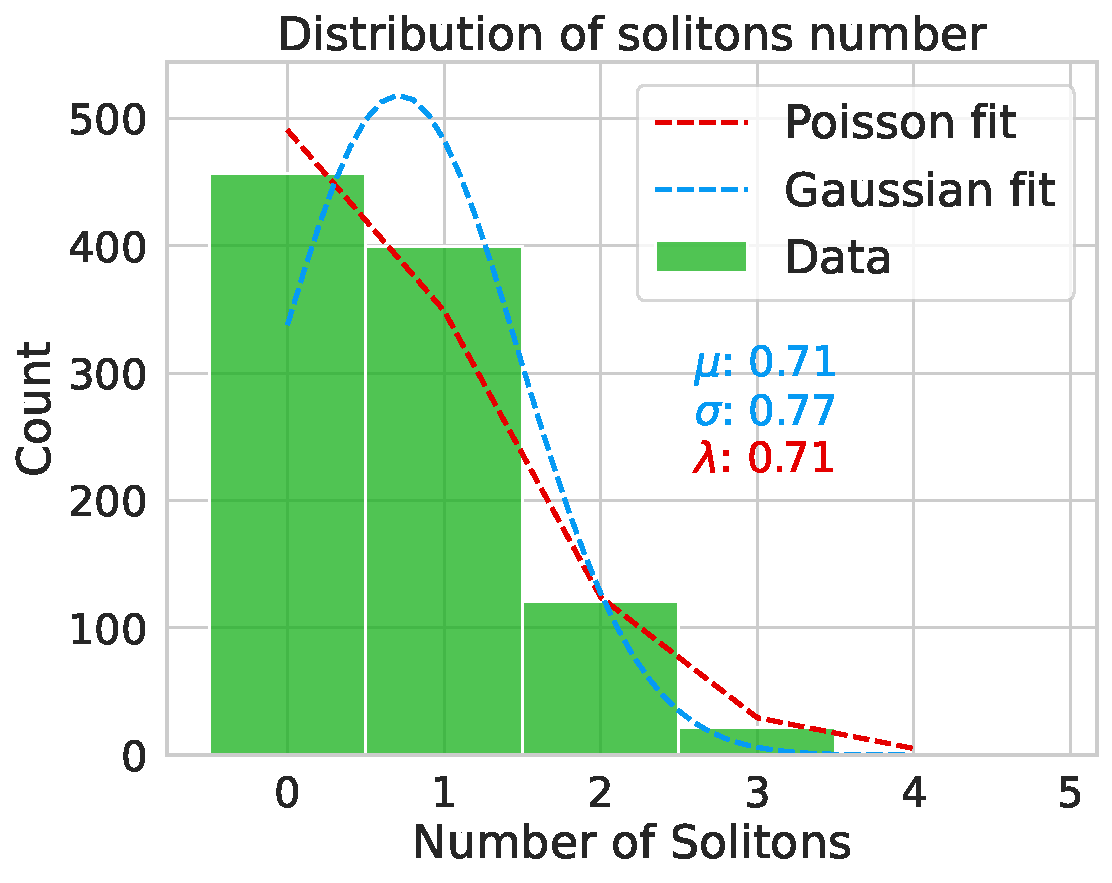
\includegraphics[width=1\linewidth]{images/soliton/ds_distribution_poisson.pdf}
    }
    \end{minipage}
    \hfill
    \begin{minipage}[h]{0.49\linewidth}
    \center{
        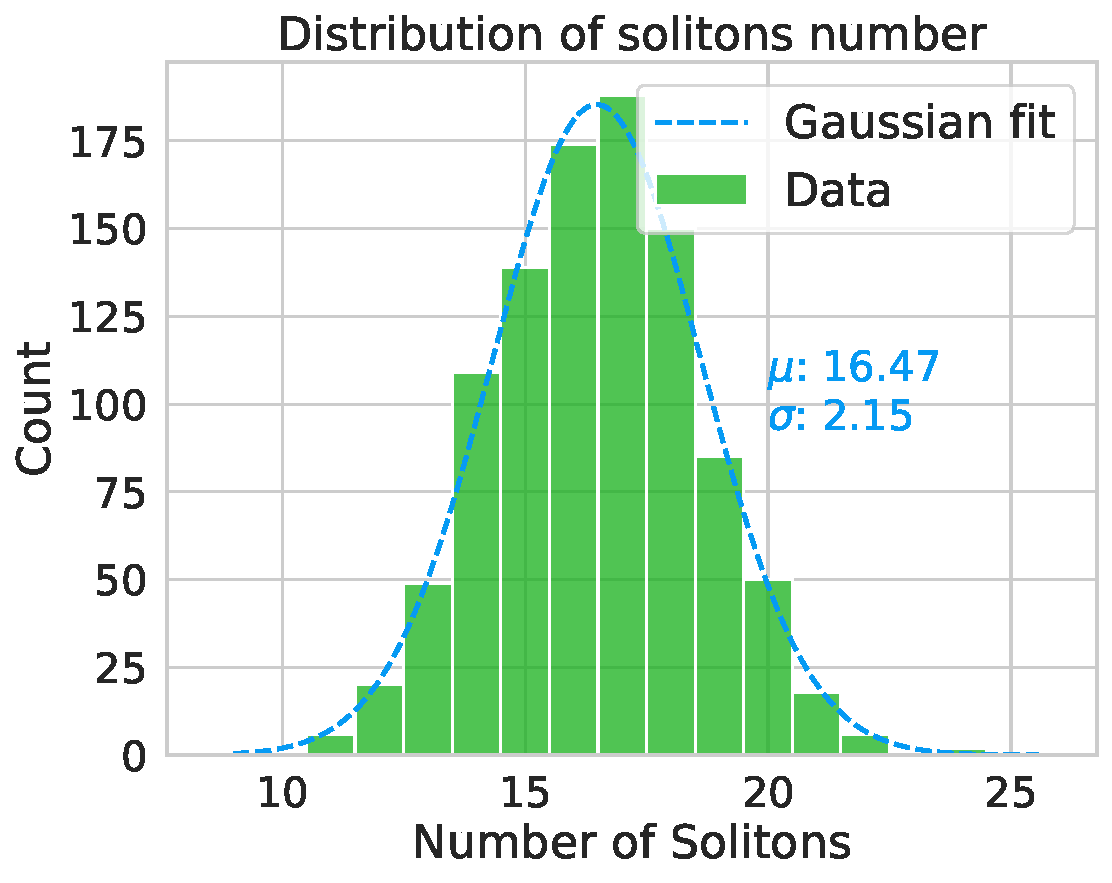
\includegraphics[width=1\linewidth]{images/soliton/ds_distribution_gauss.pdf}
    }
    \end{minipage}
    \caption{The probability of soliton occurrence in an OFDM signal with QPSK modulation, 64 subcarriers and an average power of -20 dBm \textbf{(left)} and -15 dBm \textbf{(right)}.}
    \label{fig:ds_stat}
\end{figure}

In general, signals may comprise multiple solitons. When the average power of a signal coincides with the soliton existence threshold, the resulting set of signals with random data may include those without solitons or those with one or more solitons. Statistical analysis of such signals yields a distribution of soliton numbers within the signal, as depicted in Fig.~\ref{fig:ds_stat}. This figure juxtaposes the fits for both Poisson ($P(x;\lambda) = e^{-\lambda} \lambda^x / x!$) and Gaussian distributions against the empirical distribution derived from simulation data. We consider $1000$ signal events for this analysis.

The left panel of Fig.~\ref{fig:ds_stat} corresponds to the boundary case, where a subset of the signals contains no solitons. Conversely, the right panel represents scenarios where solitons are always present in the signal, given certain parameters, though their number varies with the initial data. In such instances, the Gaussian distribution, denoted as $G(x) = \frac{1}{\sigma \sqrt{2 \pi}} e^{-\frac{(x-\mu)^2}{2\sigma^2}}$, where $\mu$ is the mean and $\sigma$ is the standard deviation, provides an accurate model of the distribution.


In the first phase of our study, we focus exclusively on the occurrence of solitons within the signal. Notably, we quantify the presence of solitons rather than their quantity or individual properties. Consequently, we define the probability of a discrete spectrum's presence as the proportion of signals containing at least one soliton relative to the total number of signals with specific parameters.

The signal's average power, denoted as \( P_{\text{ave}} \), correlates with the \( L_2 \) norm (see Equation~\ref{eq:l2}) through the relationship \( P_{\text{ave}} = \frac{L_2}{T} \), where \( T \) represents the symbol interval, the duration of a single symbol. Power measurements adopt milliwatts (mW) and decibels-milliwatts (dBm), with the conversion given by \( P_{\text{dBm}} = 10 \log_{10}(P_{\text{mW}}) \).

For our numerical simulations, we apply specific optical fiber parameters: the group velocity dispersion \( \beta_2 = -21.5 \ \text{ps}^2/\text{km} \) and the Kerr nonlinearity coefficient \( \gamma = 1.27 \ \text{W}^{-1}/\text{km} \). It is crucial to note that at this stage, we have not considered signal propagation, meaning our analysis pertains solely to the initial conditions, framing it as a Cauchy problem for the \gls{nlse}.



\begin{figure}[htpb]
    \center{
        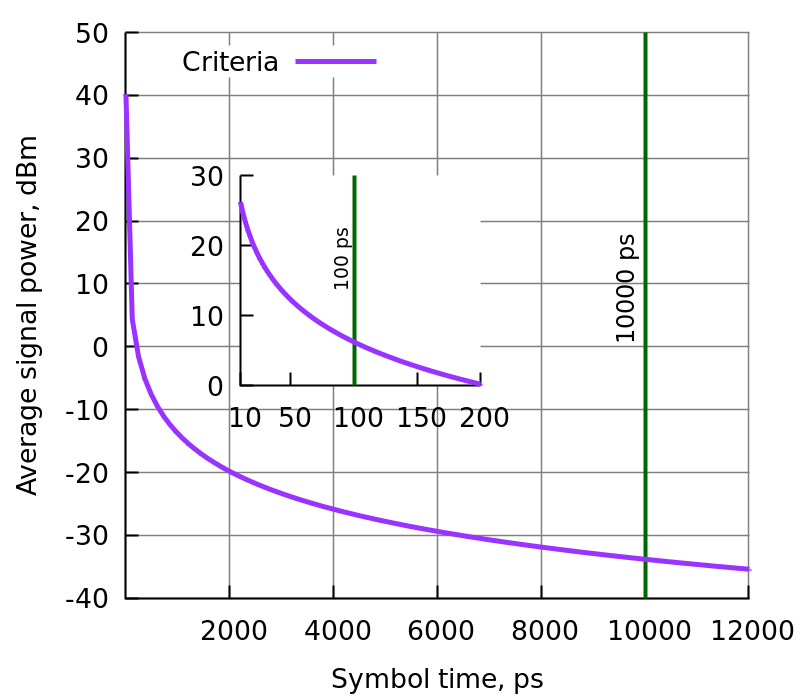
\includegraphics[width=0.5\linewidth]{images/soliton/criteria.png}
    }
    \caption{The dependence of the criteria~(\ref{eq:pave_criteria}) in dimensional units on the symbol duration $ T $.}
    \label{fig:criteria_dim}
\end{figure}

To ascertain the operational ranges for optical signals, we reference the soliton existence criterion as expressed in Eq.~\eqref{eq:l2_criteria}, given in dimensional form by
\begin{equation}
    P_{\text{ave}} > \frac{|\beta_2| \pi^2}{4\gamma T_s^2},
    \label{eq:pave_criteria}
\end{equation}
where \( T_s \) denotes the interval of interest, equivalent to the duration of a single symbol in OFDM or WDM signaling. Figure~\ref{fig:criteria_dim} illustrates the relationship between the minimum average power necessary for the potential existence of a discrete spectrum and the symbol duration. The symbol durations examined herein are highlighted by green lines. For instance, at 10 ns, the threshold lies below -30 dBm (specifically, -33.8 dBm), whereas at 100 ps, the requisite threshold significantly increases to 6.2 dBm. These thresholds guide the selection of appropriate power levels for examining each signal type. Notably, the graph displays the aggregate average power; however, in the context of WDM systems, the average power per channel is typically the metric of interest. This distinction is accounted for in subsequent recalculations.



\subsection{OFDM symbol}

\begin{figure}[htpb]
    \center{
        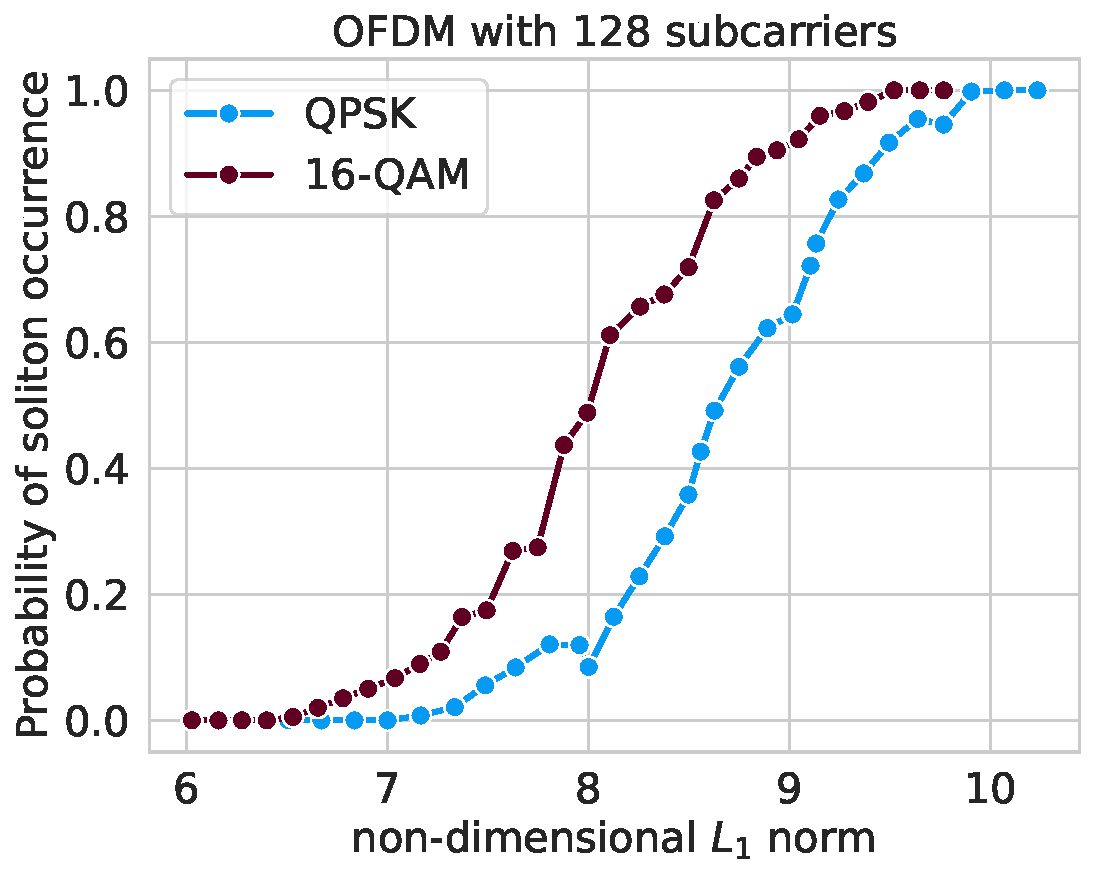
\includegraphics[width=0.47\linewidth]{images/soliton/ofdm_vs_l1.pdf}
    }
    \caption{Dependence of the probability of soliton occurrence in OFDM signals with 128 subcarriers and QPSK and 16-QAM modulation.}
    \label{fig:ofdm_result_1}
\end{figure}

The mathematical formulation of an OFDM symbol generation is detailed in Section~\ref{sec:ofdm}, specifically in Equation~\ref{eq:ofdm_symbol}. Dimensionally, we investigate OFDM symbols with a duration of 10 ns and modulation schemes including QPSK, 16-QAM, 64-QAM, and 1024-QAM. The count of subcarriers ranges from 16 to 1024, with a full Fast Fourier Transform (FFT) size of 1024. Initially, our analysis sought to determine if soliton numbers within a signal were affected by changes in FFT size. Our findings indicate that the soliton count remains invariant, provided the FFT size is fixed at 128.

Further analysis was conducted on 200 simulated symbols with random input data, holding the parameters constant for each point graphed. The Mersenne Twister algorithm, mt19937, was utilized for generating 32-bit pseudo-random numbers with a 19937-bit state size. Figure~\ref{fig:ofdm_result_1} presents the correlation between the probability of soliton formation in a signal and the \( L_1 \) norm, for a configuration with 128 subcarriers modulated by QPSK and 16-QAM. The baseline \( L_1 \) norm value, calculated as per Equation~\ref{eq:n_soliton_l1} and equal to 1.57, falls outside the left margin of the graph. In subsequent sections, the paper delves into the dependency of soliton existence probability on the average power of the signal, as this measure has a direct physical interpretation and can be measured experimentally.


\begin{figure}[htpb]
    \begin{minipage}[h]{0.47\linewidth}
        \center{
            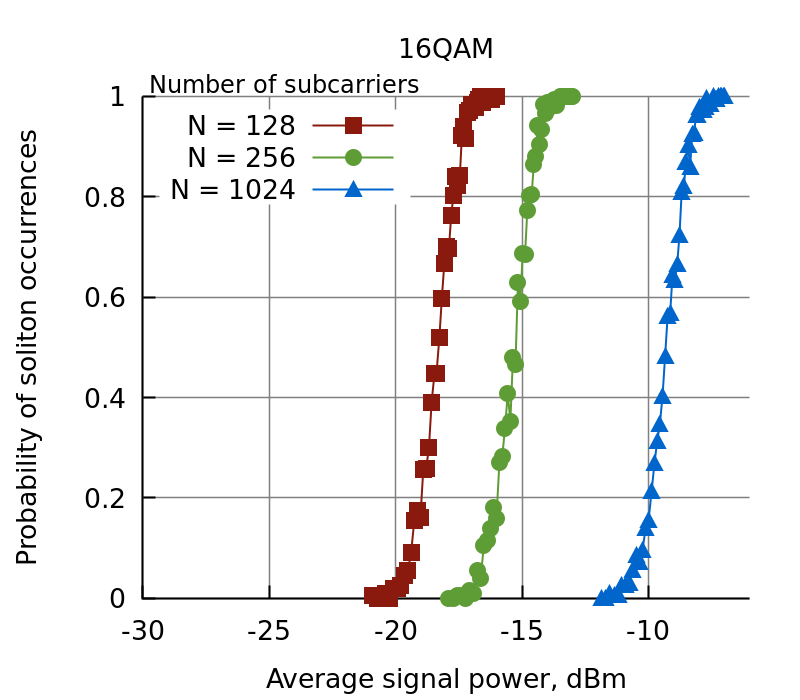
\includegraphics[width=1\linewidth]{images/soliton/10ns_ofdm_prob_16qam.png} a) \\
        }
    \end{minipage}
    \hfill
    \begin{minipage}[h]{0.47\linewidth}
        \center{
            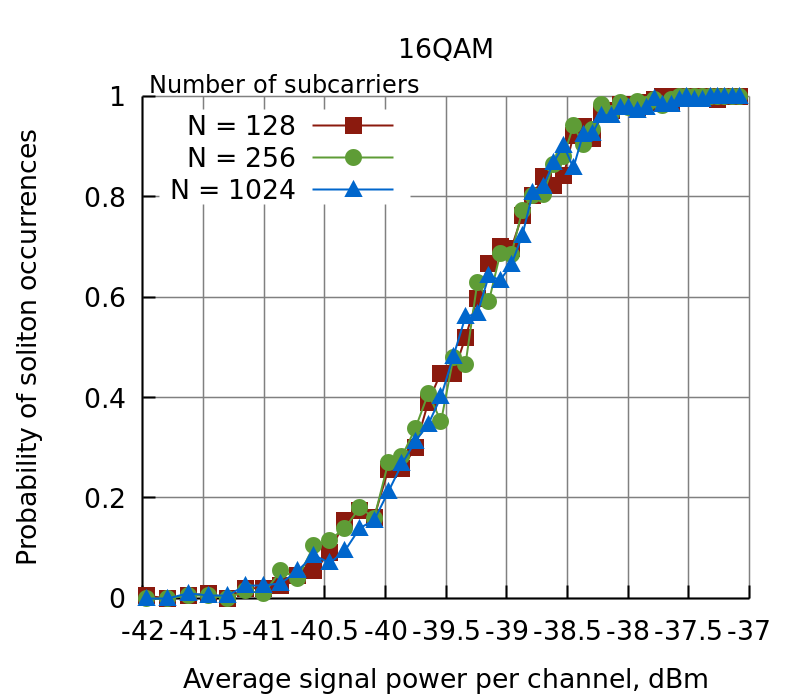
\includegraphics[width=1\linewidth]{images/soliton/10ns_ofdm_prob_ch_16qam.png} b) \\
        }
    \end{minipage}

    \caption{The dependence of the probability of soliton occurrence for OFDM signals with 16-QAM and a symbol duration of 10 ns from (a) on average signal power, (b) on average signal power per channel.}
    \label{fig:ofdm_result_16qam}
\end{figure}

Figure~\ref{fig:ofdm_result_16qam}(a) displays the relationship between the probability of soliton presence in OFDM signals with 16-QAM modulation and the average signal power. It is observed that as the number of subcarriers increases, so does the required power for soliton formation. This effect can be explained in Figure~\ref{fig:ofdm_result_16qam} (b), which presents a corresponding graph considering that the average power is distributed across each individual subcarrier. This plot clarifies that the probability of soliton existence is actually governed by the power density within each subcarrier, independent of the total number of subcarriers. Consequently, an augmentation in the number of subcarriers necessitates a proportional increase in overall signal power to sustain soliton presence. Same trends are detected for different modulation schemes, as depicted in Figure~\ref{fig:ofdm_result_mod_all}. The findings suggest that the operational power bandwidth per channel conducive to solitons lies between \(-42\) dBm and \(-37\) dBm. Leveraging this insight allows us to approximate the soliton existence thresholds for varied signal configurations.


\begin{figure}[htpb]
    \begin{minipage}[h]{0.47\linewidth}
        \center{
            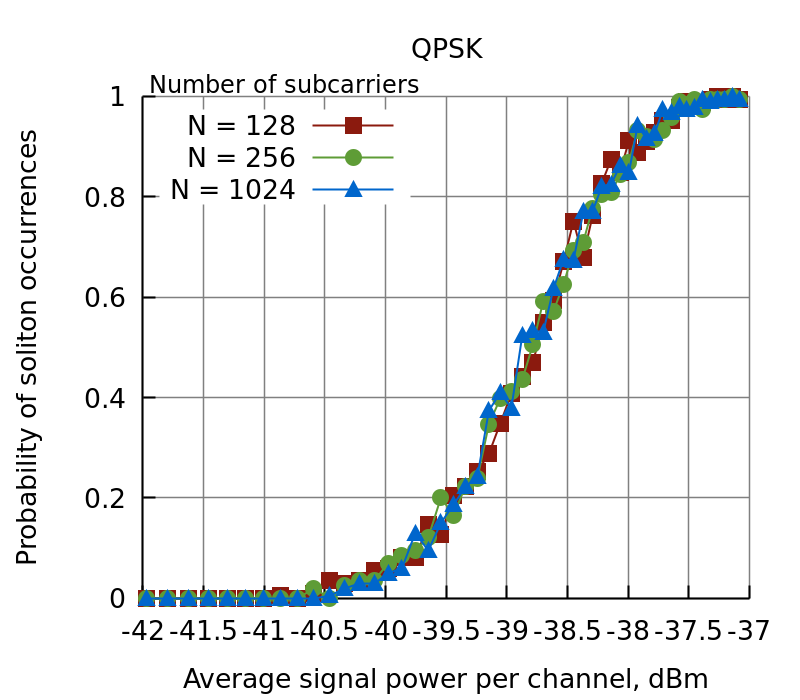
\includegraphics[width=1\linewidth]{images/soliton/10ns_ofdm_prob_ch_qpsk.png} a) \\
        }
    \end{minipage}
    \hfill
    \begin{minipage}[h]{0.47\linewidth}
        \center{
            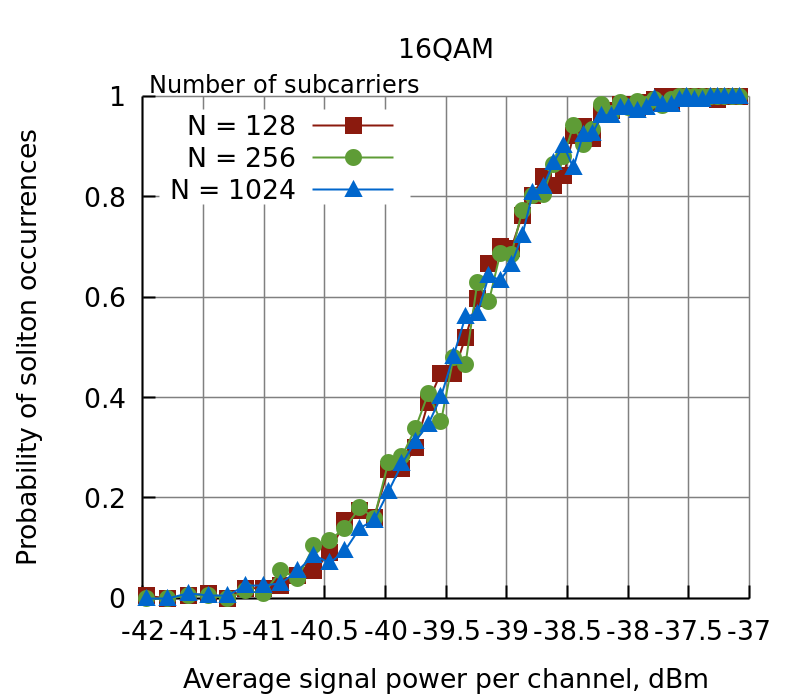
\includegraphics[width=1\linewidth]{images/soliton/10ns_ofdm_prob_ch_16qam.png} b) \\
        }
    \end{minipage}
    \vfill
    \begin{minipage}[h]{0.47\linewidth}
        \center{
            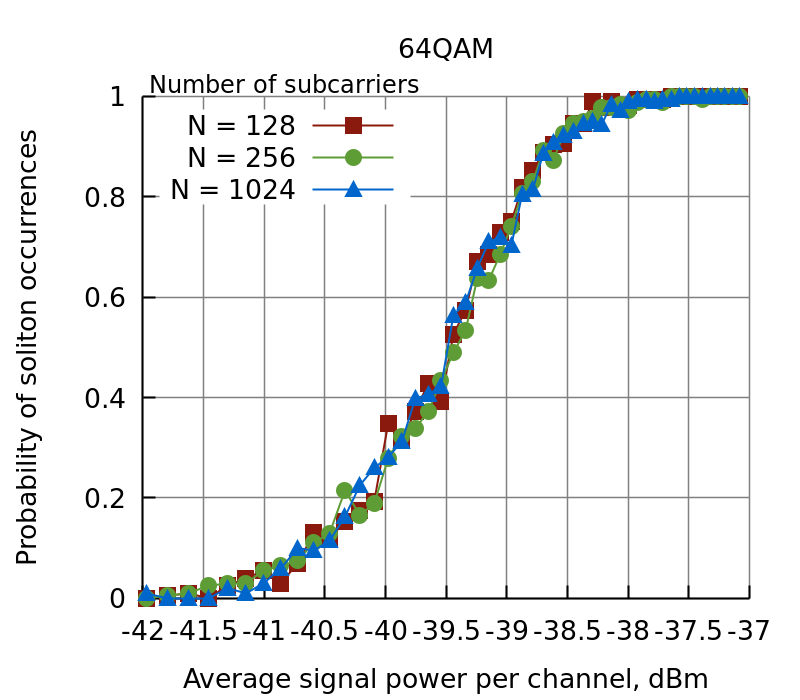
\includegraphics[width=1\linewidth]{images/soliton/10ns_ofdm_prob_ch_64qam.png} c) \\
        }
    \end{minipage}
    \hfill
    \begin{minipage}[h]{0.47\linewidth}
        \center{
            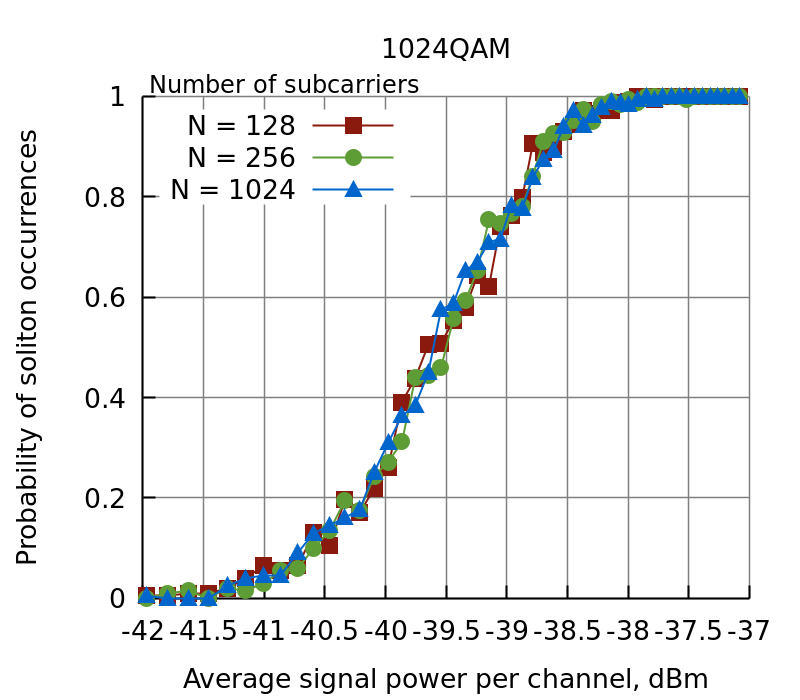
\includegraphics[width=1\linewidth]{images/soliton/10ns_ofdm_prob_ch_1024qam.png} d) \\
        }
    \end{minipage}

    \caption{The dependence of the probability of soliton occurrence in the OFDM symbol with a duration of 10 ns and (a) QPSK, (b) 16-QAM, (c) 64-QAM, (d) 1024-QAM modulation on the average signal power per channel.}
    \label{fig:ofdm_result_mod_all}
\end{figure}

However, the type of modulation also affects the probability distribution. Figure~\ref{fig:ofdm_result_sub_all} demonstrates that with an increase in the order of the constellation diagram, and hence with an increase in the number of bits of information encoded in one symbol, the required average signal power for the existence of solitons decreases. This fact is well seen when comparing QPSK and other types of modulation. Irrespective of the number of subcarriers, there is a tendency that for QPSK modulation, the average signal power is higher than for others. If we proceed to the dependence on the average power per channel, the situation will not change (Fig.~\ref{fig:ofdm_result_sub_128}).

\begin{figure}[htpb]
    \begin{minipage}[h]{0.47\linewidth}
        \center{
            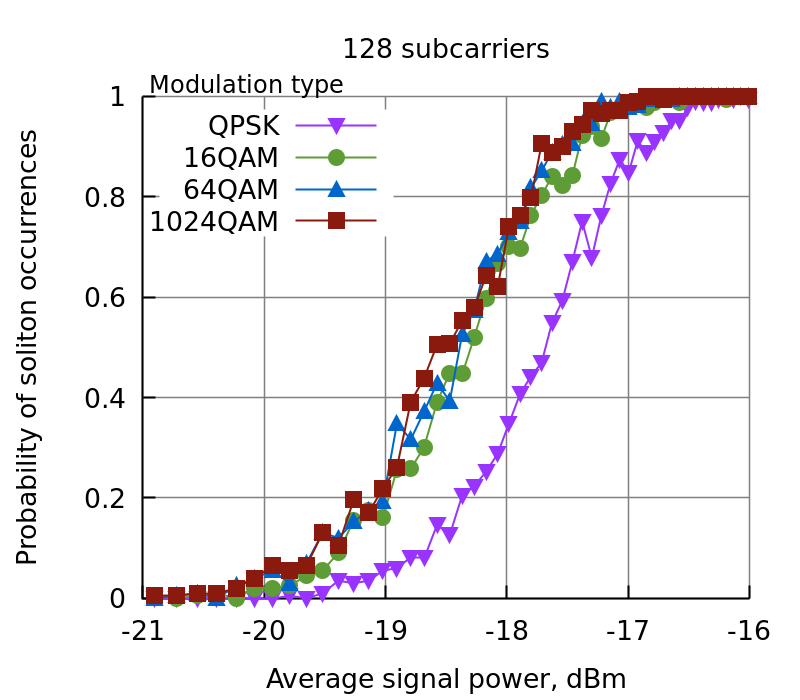
\includegraphics[width=1\linewidth]{images/soliton/10ns_ofdm_prob_128.png} a) \\
        }
    \end{minipage}
    \hfill
    \begin{minipage}[h]{0.47\linewidth}
        \center{
            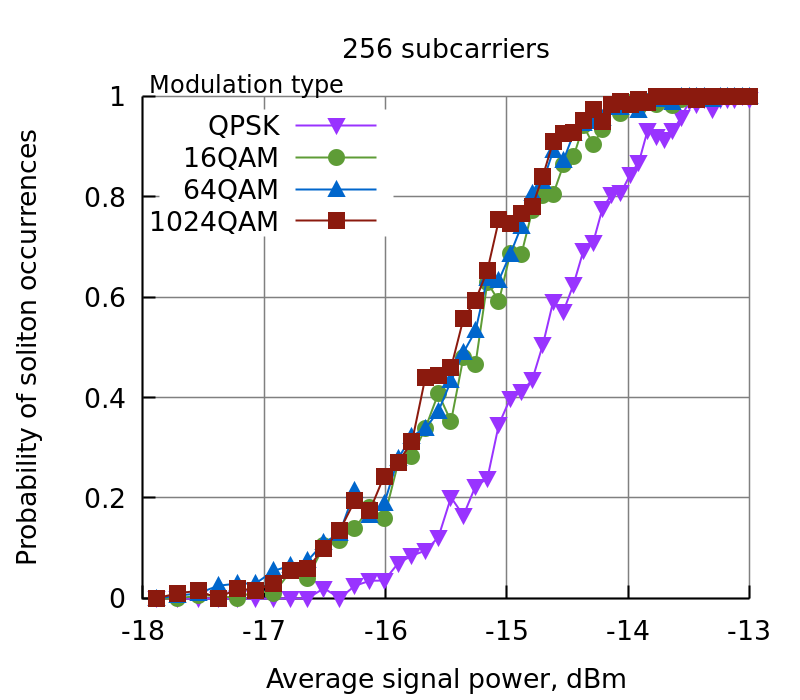
\includegraphics[width=1\linewidth]{images/soliton/10ns_ofdm_prob_256.png} b) \\
        }
    \end{minipage}
    \vfill
    \center{
        \begin{minipage}[h]{0.47\linewidth}
            \center{
                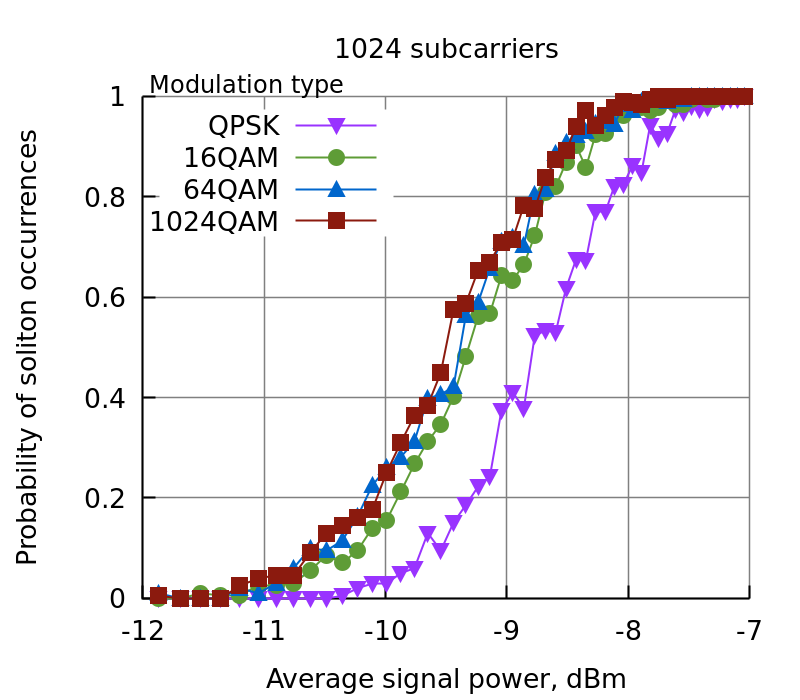
\includegraphics[width=1\linewidth]{images/soliton/10ns_ofdm_prob_1024.png} c) \\
            }
        \end{minipage}
    }

    \caption{The dependence of the probability of soliton occurrence in the OFDM symbol with a duration of 10 ns and (a) 128, (b) 256, (c) 1024 subcarriers on the average signal power.}
    \label{fig:ofdm_result_sub_all}
\end{figure}

\begin{figure}[htpb]
    \center{
        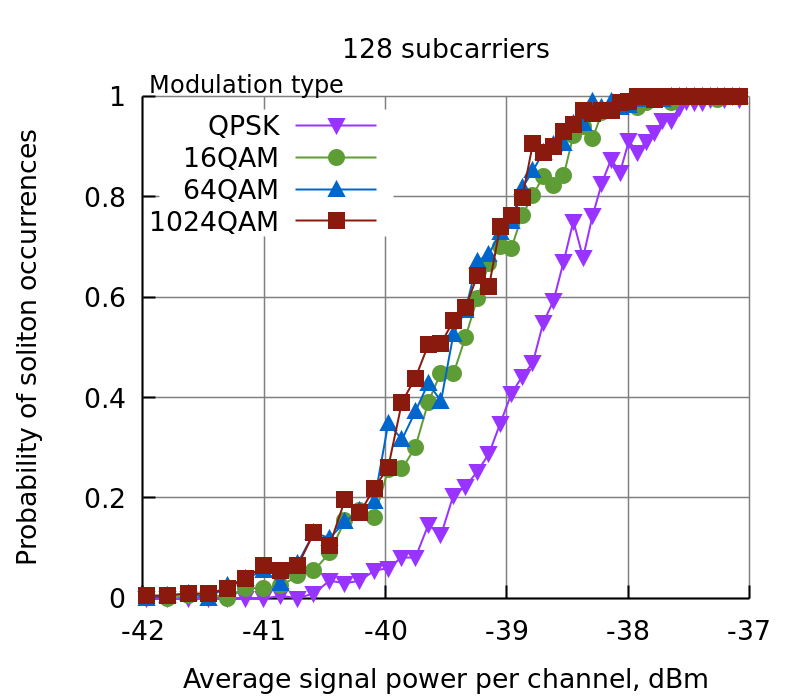
\includegraphics[width=0.47\linewidth]{images/soliton/10ns_ofdm_prob_ch_128.png}
    }
    \caption{The dependence of the probability of soliton occurrence in the OFDM symbol with a duration of 10 ns and 128 subcarriers on the average signal power per channel.}
    \label{fig:ofdm_result_sub_128}
\end{figure}

As expected, for a complex signal the level of $L_1$ and $L_2$ norms (and hence $P_ {ave}$), at which solitons exist in the signal, is higher than for a simple rectangular signal. This is consistent with the criteria~(\ref{eq:pave_criteria}), which can also be used for preliminary analysis in other existing systems. 

In the general case, solitons and dispersion waves propagate through the fiber in different ways. The most important difference is that the dispersion for solitons is balanced by nonlinear effects. The existence of solitons in a standard OFDM signal has the potential to make some contribution in propagation. Understanding of this fact may affect coding and modulation of signals in optical communication, as it can lead to an improvement in the efficiency of optical communication lines. However, in practice, the appearance of solitons does not have a large effect on the propagation dynamics of the OFDM signal at the considered power levels. At higher levels, it is already possible to observe the evolution of individual solitons in a common signal, however, these events are rare, and more research is needed to determine the parameters and degree of influence of solitons on the signal.

\clearpage

\subsection{WDM symbol} 

\Gls{wdm} technology enables the simultaneous transmission of multiple data channels through a single optical fiber, each at a different frequency. \Gls{wdm} works by sending information on various wavelengths within the same fiber-optic line, with each wavelength known as a "channel," a term we will use throughout.

Data is transmitted using a specific modulation format. The carrier frequency for each channel, \(f_n\), is determined by the formula:
\begin{equation}
    f_n = \Delta \cdot n, \quad n = -N/2 \ldots N/2,
\end{equation}
where \( \Delta \) represents the spacing between channels, which in this case is set to 25 GHz as detailed in Eq.~(\ref{eq:wdm_nlse}). The duration of one symbol is 100 ps.


At this point, we're looking at WDM signals that use different modulation formats such as QPSK, and 16-, 64-, and 1024-QAM. We also vary the number of channels from 9 to 51. Just like we did with OFDM signals, we gathered data on 200 WDM symbols for every combination of parameters. Figure~\ref{fig:wdm_result_mod_all} displays the probability of existence in a signal, depending on the average power per channel for different types of modulation and different number of channels. It's important to note that these measurements are for power in each WDM channel, not the total power across all channels.

\begin{figure}[htpb]
    \begin{minipage}[h]{0.47\linewidth}
        \center{
            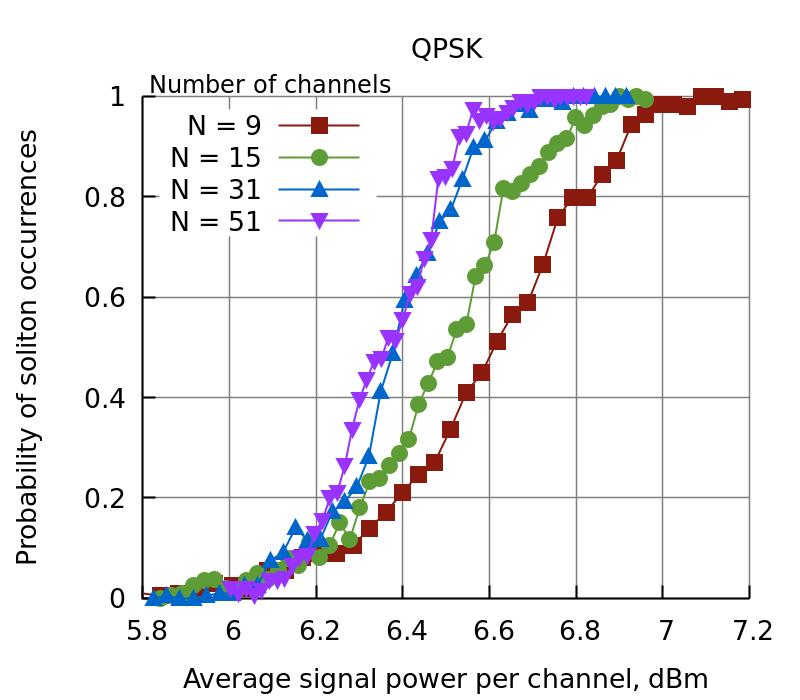
\includegraphics[width=1\linewidth]{images/soliton/100ps_prob_ch_result_qpsk.png} a) \\
        }
    \end{minipage}
    \hfill
    \begin{minipage}[h]{0.47\linewidth}
        \center{
            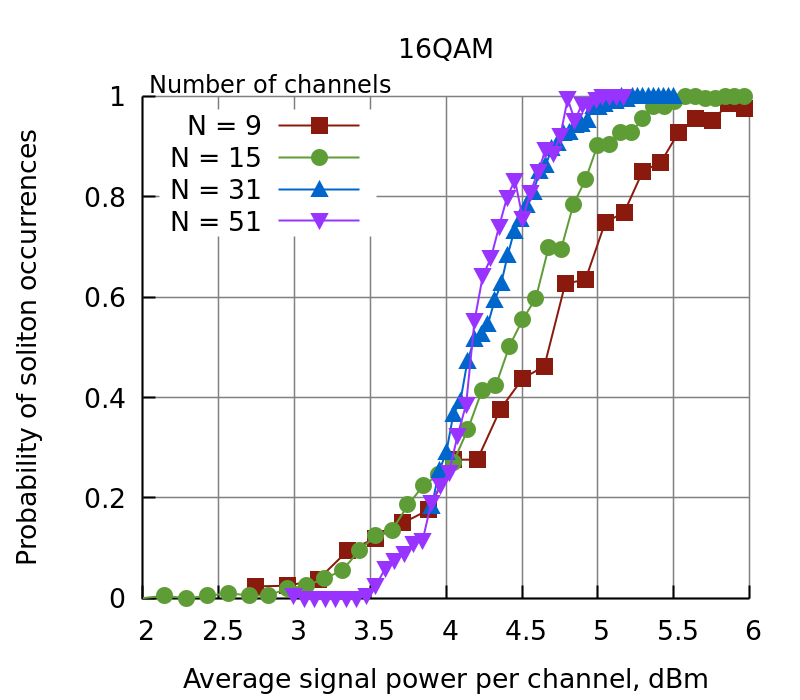
\includegraphics[width=1\linewidth]{images/soliton/100ps_prob_ch_result_16qam.png} b) \\
        }
    \end{minipage}
    \vfill
    \begin{minipage}[h]{0.47\linewidth}
        \center{
            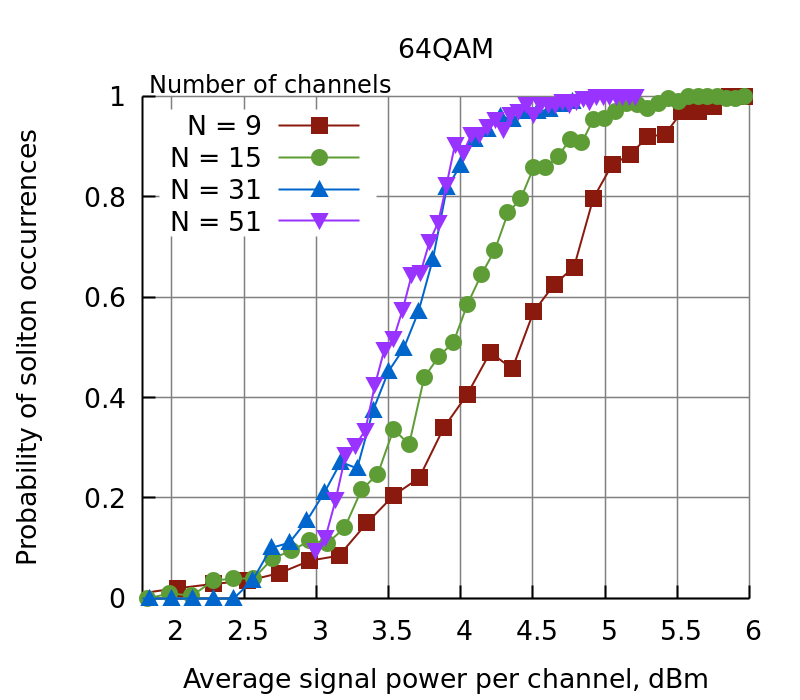
\includegraphics[width=1\linewidth]{images/soliton/100ps_prob_ch_result_64qam.png} c) \\
        }
    \end{minipage}
    \hfill
    \begin{minipage}[h]{0.47\linewidth}
        \center{
            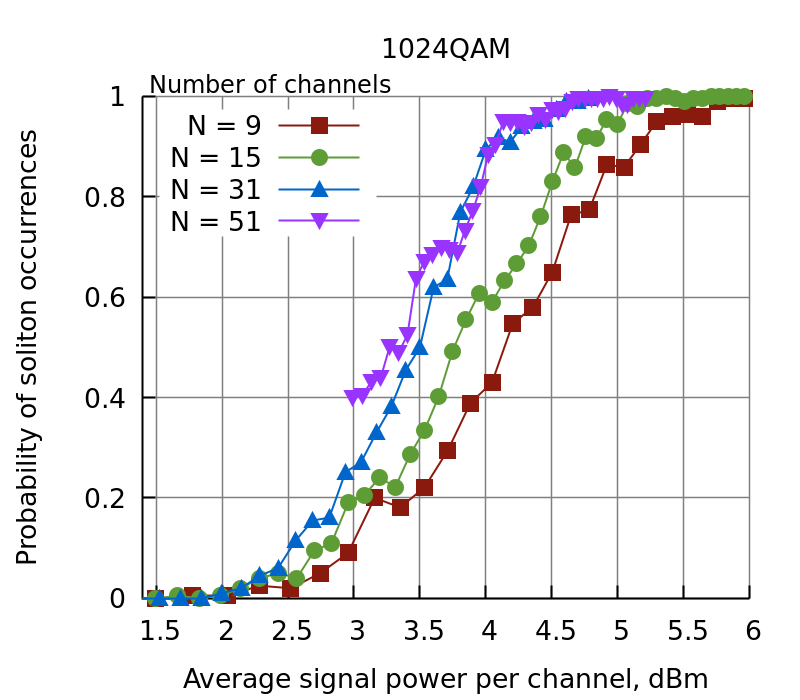
\includegraphics[width=1\linewidth]{images/soliton/100ps_prob_ch_result_1024qam.png} d) \\
        }
    \end{minipage}

    \caption{The dependence of the probability of solitons occurrence in a WDM signal on the average signal power per channel with a duration of 100 ps and (a) QPSK, (b) 16-QAM, (c) 64-QAM, (d) 1024-QAM modulation.}
    \label{fig:wdm_result_mod_all}
\end{figure}

When we look at the chart in Fig.~\ref{fig:wdm_result_mod_all} (a), we see that for QPSK modulation, the necessary power level is quite a bit higher—between 5.8 dBm and 7 dBm—compared to other modulations. For 16-, 64-, and 1024-QAM, this range is broader: from 2 dBm to 6 dBm. As we use more channels, the minimum power needed tends to go down, and this reduction is consistent across all modulation types. Just like with OFDM signals, as the complexity of the modulation increases (from QPSK to 1024-QAM), the power needed to detect solitons gets lower (as shown in Fig.~\ref{fig:wdm_result_ch_all}).

Additionally, for WDM signals, QPSK modulation requires much more power compared to other modulations when it comes to finding solitons. There's also a more pronounced difference between 16-QAM, 64-QAM, and 1024-QAM for WDM signals than for OFDM signals. For instance, if we increase the number of channels to 51, the power required for 16-QAM and 64-QAM starts to diverge significantly, as depicted in Fig.~\ref{fig:wdm_result_ch_all} (d).

\begin{figure}[htpb]
    \begin{minipage}[h]{0.47\linewidth}
        \center{
            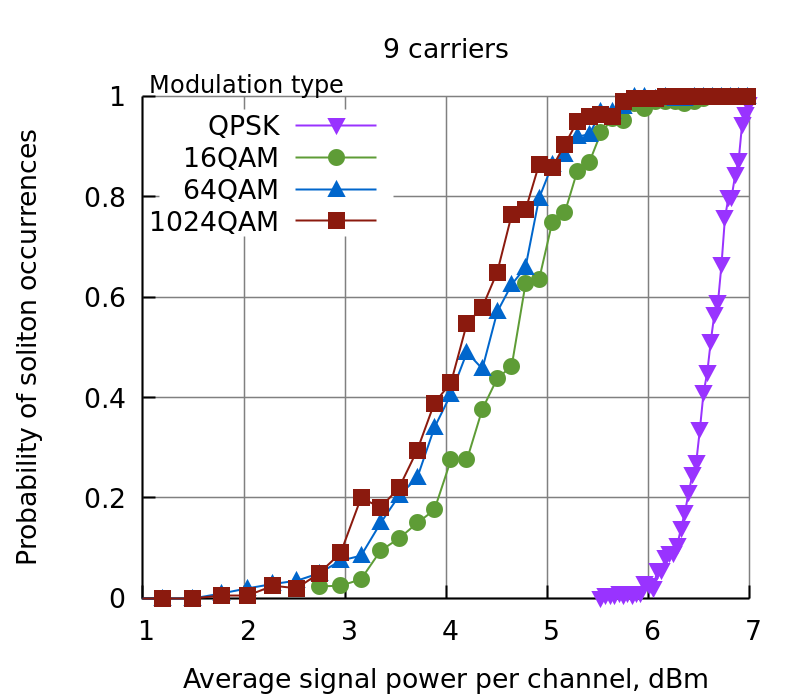
\includegraphics[width=1\linewidth]{images/soliton/100ps_prob_ch_9.png} a) \\
        }
    \end{minipage}
    \hfill
    \begin{minipage}[h]{0.47\linewidth}
        \center{
            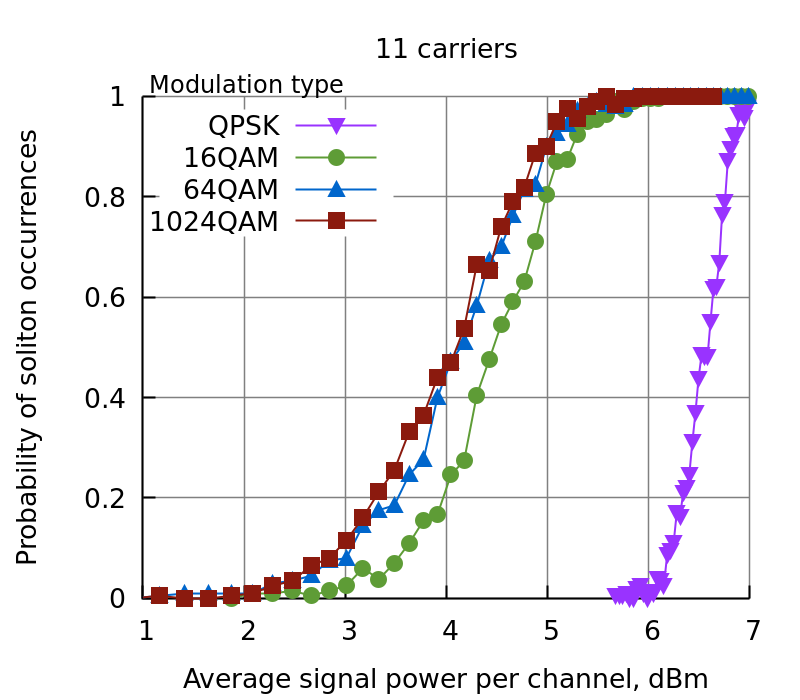
\includegraphics[width=1\linewidth]{images/soliton/100ps_prob_ch_11.png} b) \\
        }
    \end{minipage}
    \vfill
    \begin{minipage}[h]{0.47\linewidth}
        \center{
            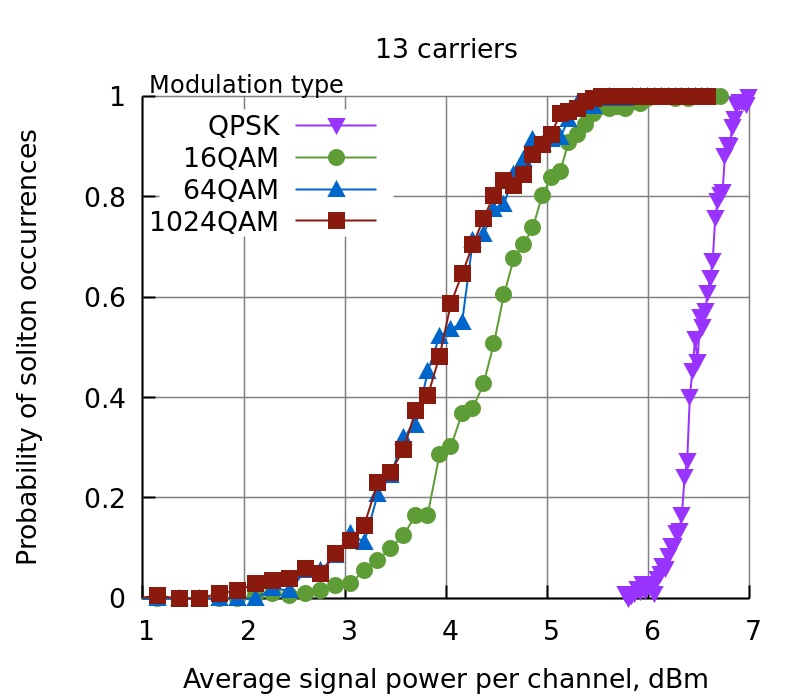
\includegraphics[width=1\linewidth]{images/soliton/100ps_prob_ch_13.png} c) \\
        }
    \end{minipage}
    \hfill
    \begin{minipage}[h]{0.47\linewidth}
        \center{
            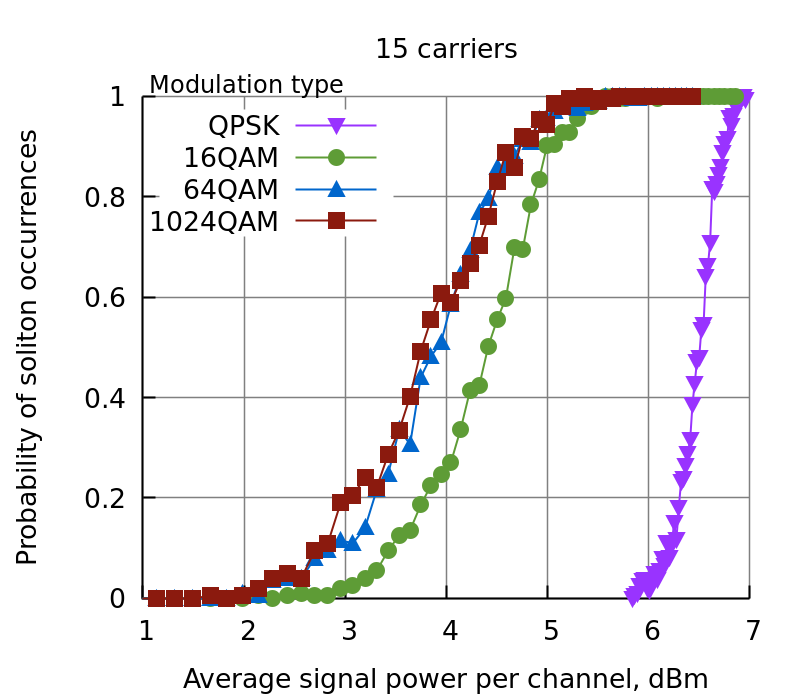
\includegraphics[width=1\linewidth]{images/soliton/100ps_prob_ch_15.png} d) \\
        }
    \end{minipage}
    \vfill
    \begin{minipage}[h]{0.47\linewidth}
        \center{
            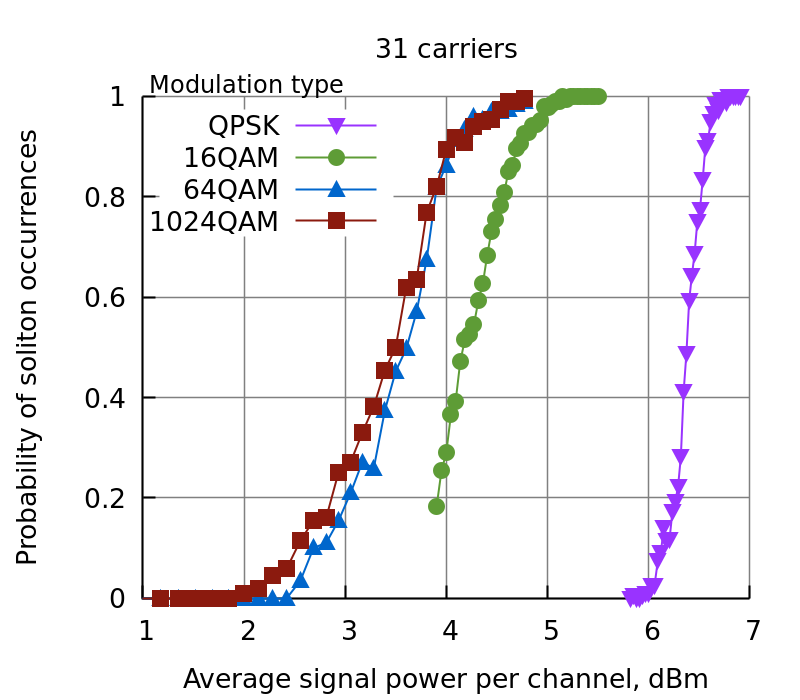
\includegraphics[width=1\linewidth]{images/soliton/100ps_prob_ch_31.png} e) \\
        }
    \end{minipage}
    \hfill
    \begin{minipage}[h]{0.47\linewidth}
        \center{
            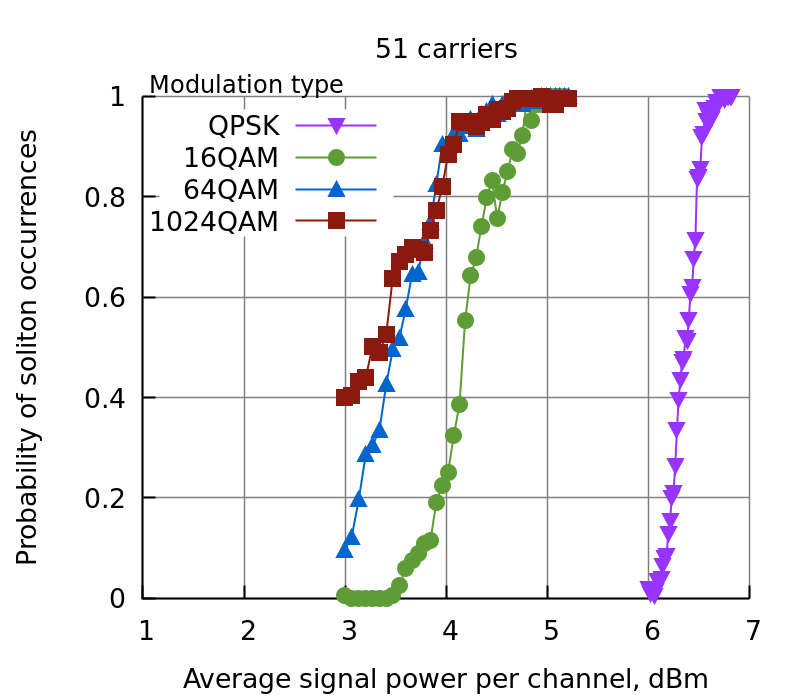
\includegraphics[width=1\linewidth]{images/soliton/100ps_prob_ch_51.png} f) \\
        }
    \end{minipage}

    \caption{The dependence of the probability of soliton occurrence in a WDM signal with (a) 9, (b) 11, (c) 13, (d) 15, (e) 31 and (f) 51 channels.}
    \label{fig:wdm_result_ch_all}
\end{figure}

These features demonstrate that, despite the similar signal generation processes, WDM and OFDM systems have a different internal structure, and also depend on the selected parameters in different ways. 

The results obtained for WDM and OFDM symbols show that coherent structures are an integral part of these systems, and therefore should be study along with other effects. The results are interesting because the features associated with nonlinearity can be evaluated and used in practice. Now, we moving forward to the analysis of more complex structuers - \gls{wdm} signals.